\documentclass[crop,tikz,convert=pdf2svg,8pt]{standalone}

% Tikz settings optimized for causal graphs.
\usetikzlibrary{shapes,decorations,arrows,calc,arrows.meta,fit,positioning}
\tikzset{
    -Latex,auto,node distance =1 cm and 1 cm,semithick ,
    state/.style ={ellipse, draw, minimum width = 0.7 cm},
    point/.style = {circle, draw, inner sep=0.04cm,fill,node contents={}},
    bidirected/.style={Latex-Latex,dashed},
    el/.style = {inner sep=2pt, align=left, sloped}
}

\begin{document}

% The graph
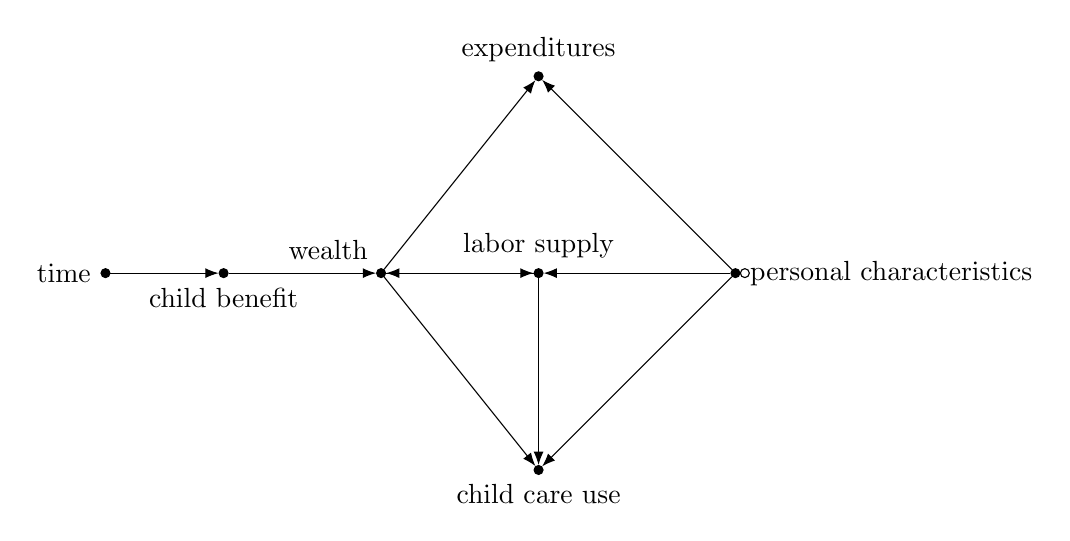
\begin{tikzpicture}
    \node (t) at (0,0) [label=left:time, point];
    \node (D) at (1.5,0) [label=below:child benefit, point];
		\node (w) at (3.5,0) [label=above left:wealth, point];
    \node (e) at (5.5,2.5) [label=above:expenditures, point];
		\node (l) at (5.5,0) [label=above:labor supply, point];
		\node (c) at (5.5,-2.5) [label=below:child care use, point];
		\node (p) at (8,0) [label=right:personal characteristics, point];
		\node (pu) at (8.12,0) [point, fill=none];

    \path (t) edge (D);
		\path (D) edge (w);
		\path (w) edge (e);
		\path (w) edge (l);
		\path (w) edge (c);
		\path (l) edge (w);
		\path (l) edge (c);
		\path (p) edge (e);
		\path (p) edge (l);
		\path (p) edge (c);
    %\path[bidirected] (2) edge[bend left=50]  (3);
\end{tikzpicture}

\end{document}